\documentclass[12pt]{beamer}

\newcommand{\insertministry}[0]{\ministry}
\newcommand{\insertchief}[0]{\chief}
\newcommand{\insertdone}[0]{\done}
\newcommand{\insertwhochiefed}[0]{\whochiefed}

\defbeamertemplate*{title page}{customized}[1][]
{
  \usebeamerfont{ministry}\insertministry\par
  \bigskip
  \bigskip
  \usebeamerfont{title}\inserttitle\par
  \usebeamerfont{subtitle}\usebeamercolor[fg]{subtitle}\insertsubtitle\par
  \bigskip
  \begin{table}
    \begin{tabular}{ p{6cm} r }
      \usebeamerfont{author}\insertdone   & \usebeamerfont{author}\insertwhochiefed \\
      \usebeamerfont{author}\insertauthor & \usebeamerfont{author}\insertchief \\
    \end{tabular}
  \end{table}
  \par
  \usebeamerfont{date}\insertdate\par
  \usebeamercolor[fg]{titlegraphic}\inserttitlegraphic
}

\usepackage[utf8]{inputenc}
\usepackage[T2A]{fontenc}
\usepackage[english,russian]{babel}

\usepackage{pscyr}          % Cyrillic fonts

% Стиль презентации
\usetheme{Szeged}
%\usefonttheme[]{serif}
\usefonttheme{professionalfonts}

\setbeamerfont{ministry}{size=\large}
\usecolortheme{lily}
\beamertemplatenavigationsymbolsempty %remove navigation symbols

\begin{document}

\def\ministry{Министерство образования и науки, молодёжи и спорта Украины}
\title{Анализ безопасности протокола WEP в компьютерных сетях стандарта 802.11~WLAN}
\def\done{Выполнил}
\author{ст.гр. БИКС-08-2\newlineФролов В.В.}
\def\whochiefed{Руководитель}
\def\chief{ст.преп. Олешко О.И.}
\date{}

% Создание заглавной страницы
\frame{\titlepage} 
% Автоматическая генерация содержания


\begin{frame}{Задачи}

    \begin{itemize}
        \item Изучить протокол WEP, процесс обмена пакетами и обеспечение аутентификации и конфиденциальности в сетях стандарта 802.11 WLAN.
        \item Исследовать возможные атаки и реализовать атаку с фрагментацией на WEP.
        \item Провести анализ безопасности WEP.
        \item Рассмотреть условия работы труда на рабочем месте и расчитать КЕО для города Харькова.
    \end{itemize}

\end{frame} 


\begin{frame}{Передача пакетов в сетях стандарта 802.11~WLAN}

    \begin{figure}
        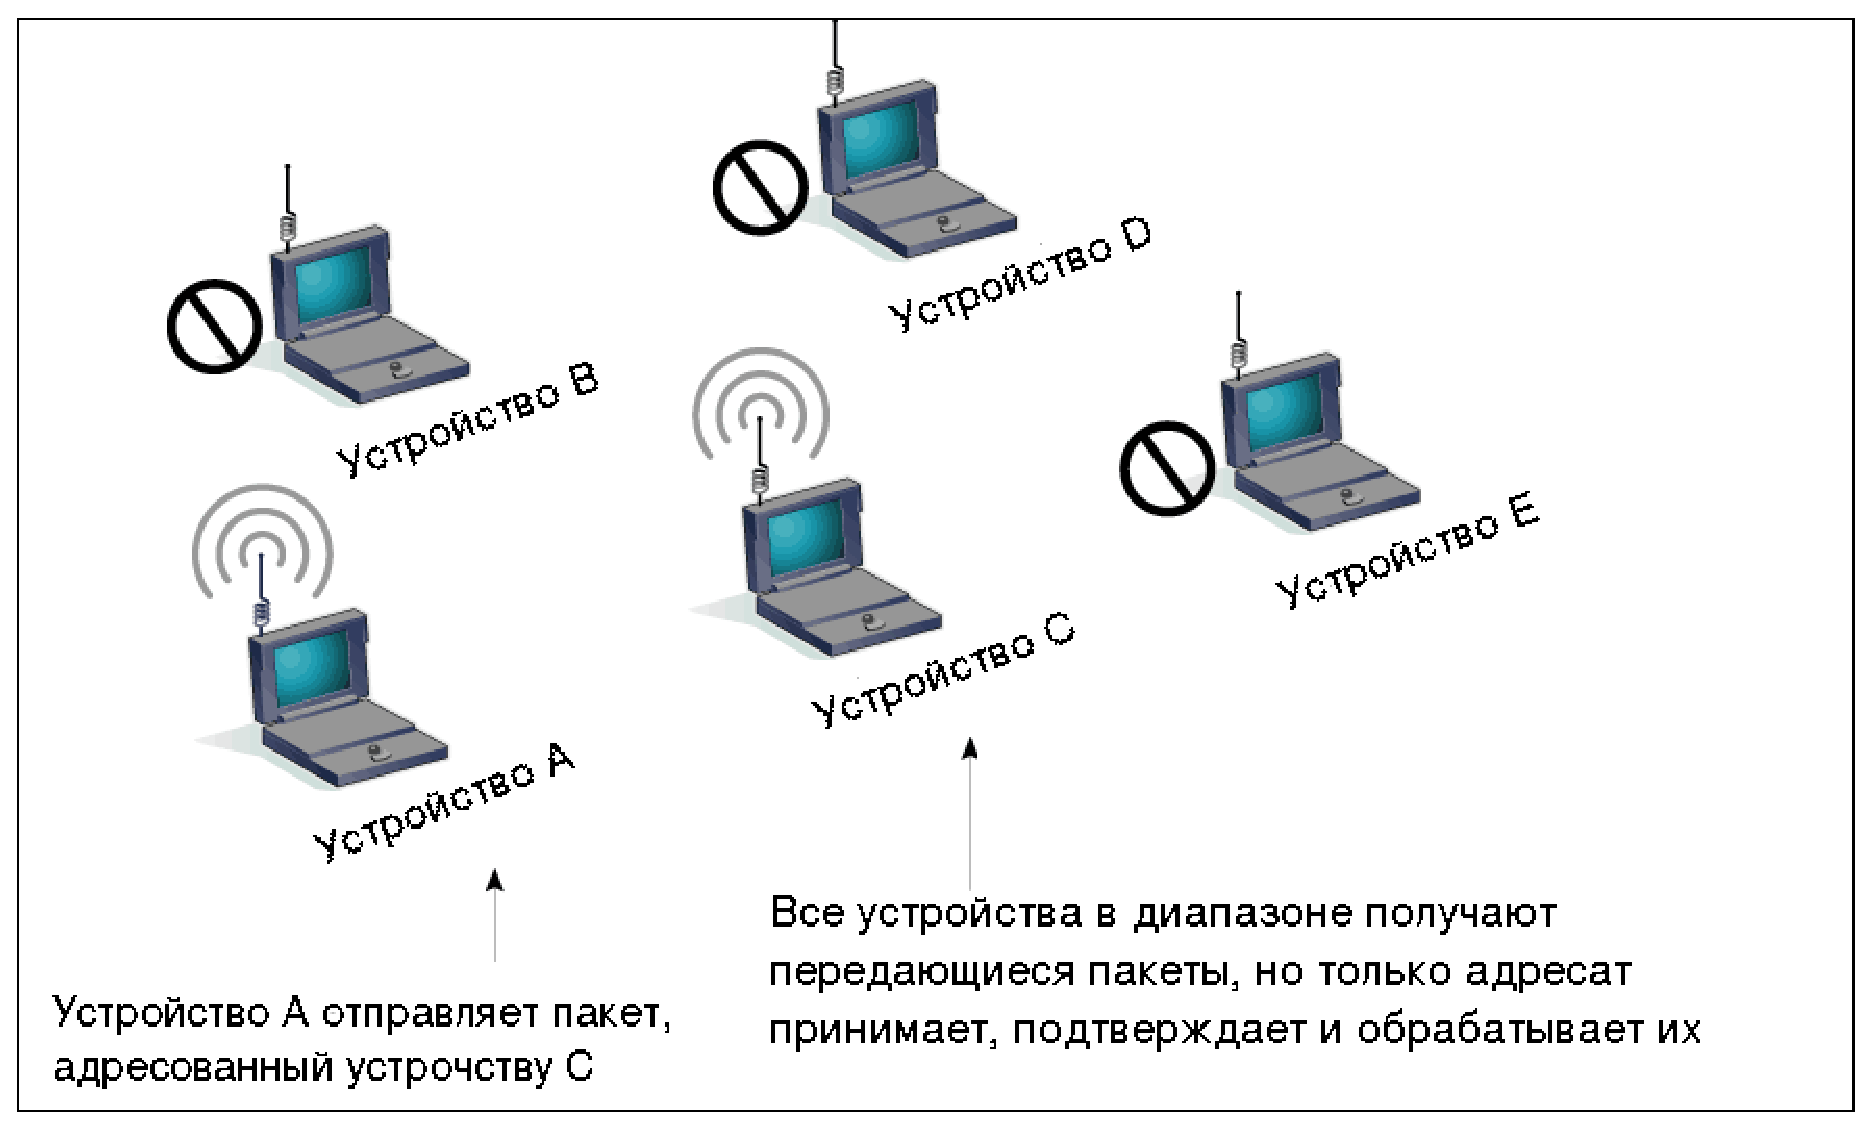
\includegraphics[width=9cm]{graphics/wlan_diagram.eps}
    \end{figure}

\end{frame} 


\begin{frame}{Нарушитель в сетях стандарта 802.11~WLAN\newline}

    \begin{figure}
        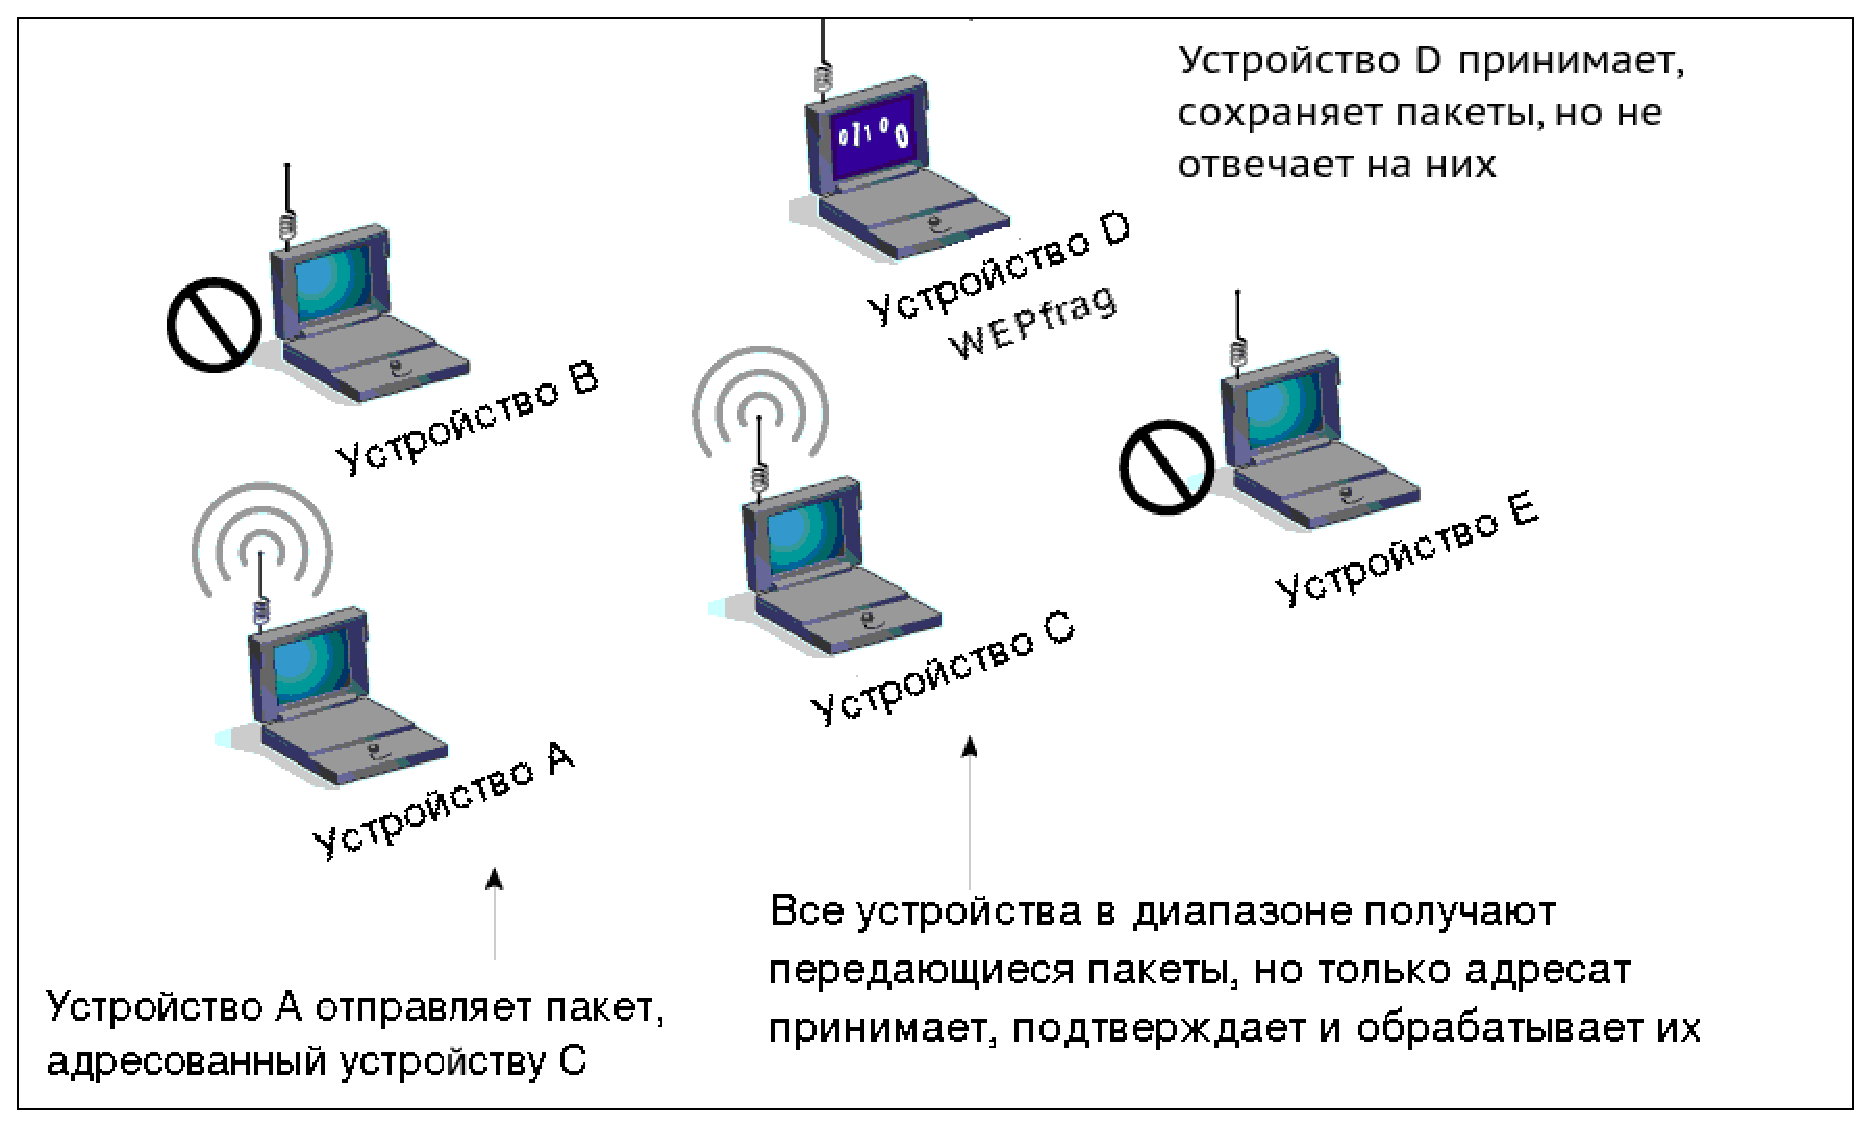
\includegraphics[width=9cm]{graphics/wlan_diagram_with_attacker.eps}
    \end{figure}

\end{frame} 


\begin{frame}{Классификация атак на протокол WEP}

    \begin{figure}
        \includegraphics[width=10cm]{graphics/wep_attacks_classification.eps}
    \end{figure}

\end{frame} 


\begin{frame}{Атака с фрагментацией}

    \begin{itemize}

        \item Вычисление ключа PRGA (шифрующей гаммы)
            \begin{figure}
                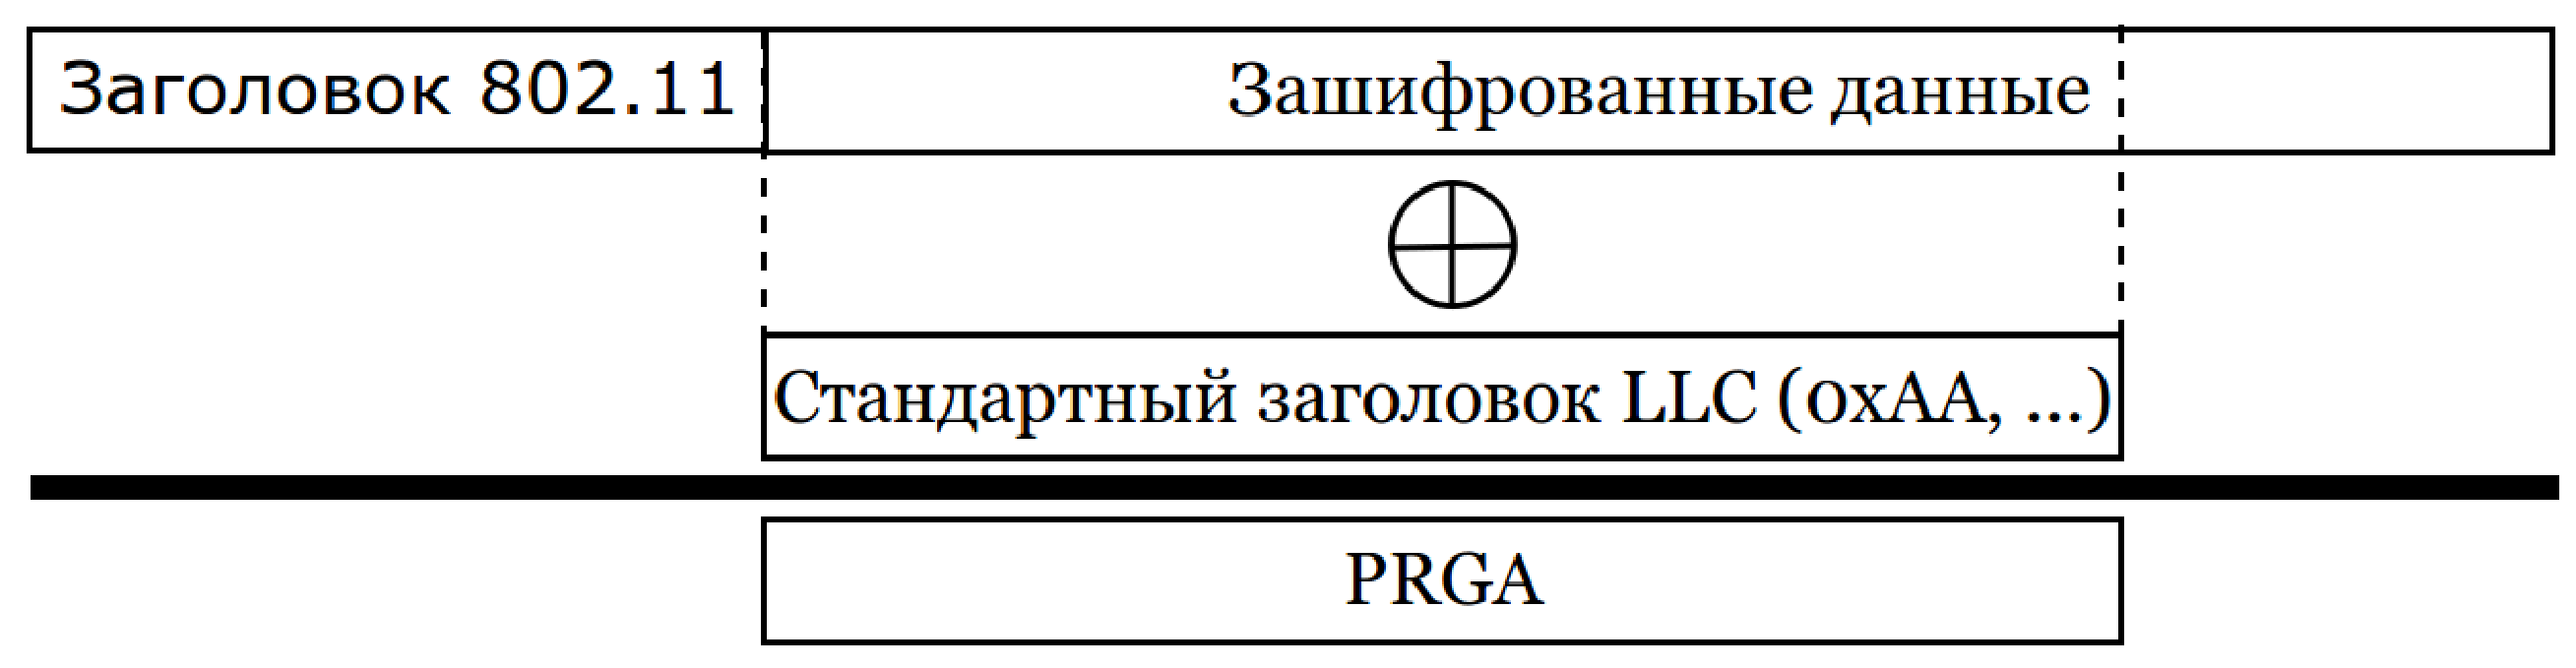
\includegraphics[width=10cm]{graphics/restore_part_of_gamma.eps}
            \end{figure}

        \item Стандартный заголовок LLC
            \begin{figure}
                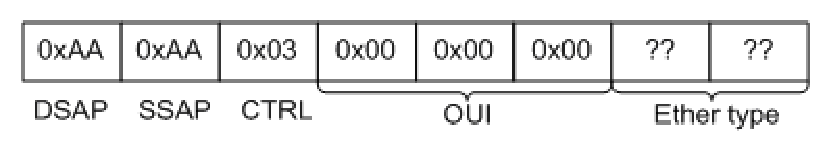
\includegraphics[width=10cm]{graphics/default_llc_header.eps}
            \end{figure}
    \end{itemize}

\end{frame} 


\begin{frame}{Алгоритм атаки с фрагментацией}

    \begin{figure}
        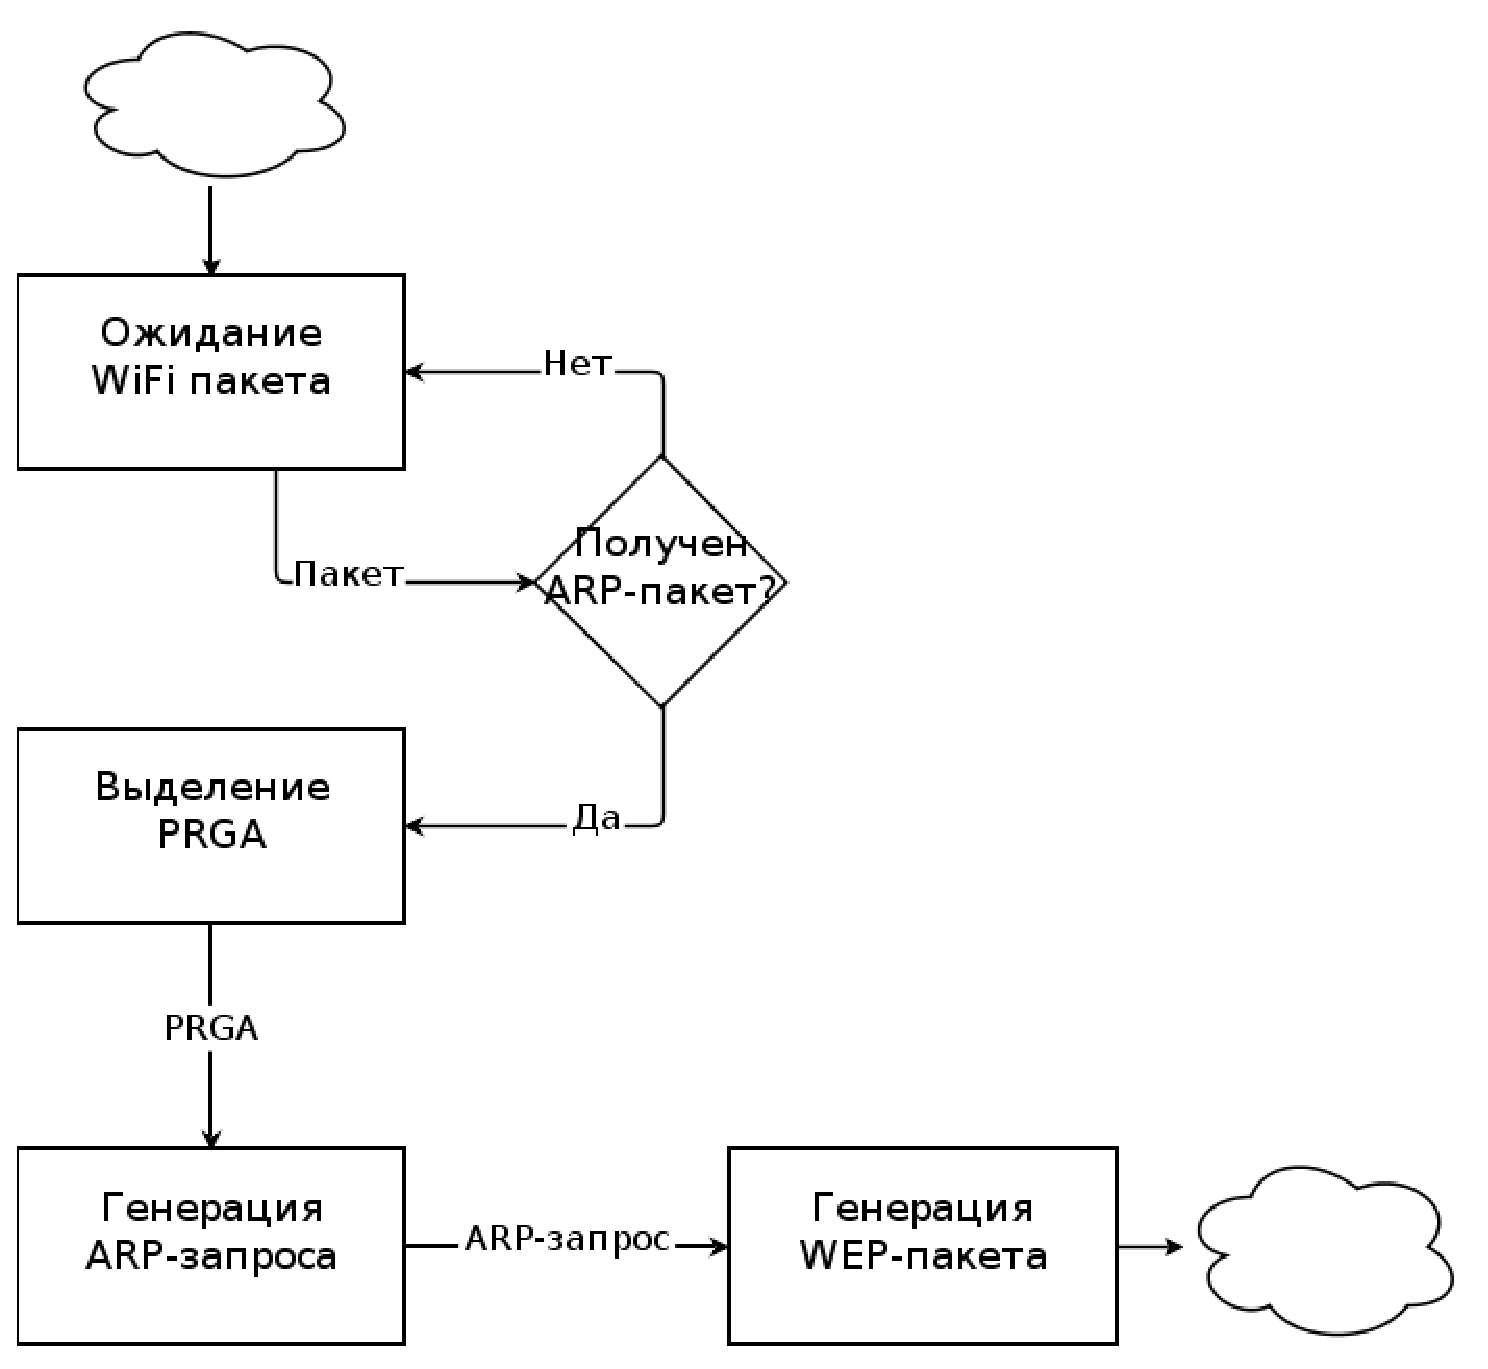
\includegraphics[width=7cm]{graphics/fragment_program_algo.eps}
    \end{figure}

\end{frame} 


\begin{frame}{Анализ безопасности протокола WEP}

    \begin{itemize}

        \item PTW атака (атака с восстановлением ключа) позволяет вычислить ключ
        в течение нескольких минут.

        \item Атака с фрагментацией (атака без восстановления ключа) позволяет
        вычислить гамму шифрования, что позволяет создавать легитимные пакеты,
        принимаемые точкой доступа.

    \end{itemize}

\end{frame} 


\begin{frame}{Охрана труда}

    \begin{itemize}
        \item Разработаны меры по охране труда в НИЛ с углублённой обработкой вопроса расчёта КЕО для города Харькова.
        \item Коэффициент естественного освещения для города Харькова составил 1,8\%.
    \end{itemize}

\end{frame} 


\begin{frame}{Выводы}

    \begin{itemize}
        \item Исследован процесс обмена пакетами и обеспечение безопасности в сетях стандарта 802.11 WLAN.
        \item Рассмотрены возможные атаки на протокол WEP.
        \item Реализована атака с фрагментацией.
        \item Проведен анализ безопасности WEP.
        \item Расчитан коэффициент естественного освещения для города Харькова.
    \end{itemize}

\end{frame} 


\begin{frame}{}

    \begin{center}
        \LARGE{Спасибо за внимание.}
    \end{center}

\end{frame}

\end{document}
